\documentclass{article}
\usepackage{graphicx}
\usepackage{leftidx}% http://ctan.org/pkg/leftidx
\graphicspath{ {images/} }

% Latex commands
    \newcommand{\mat}[2][ccccccccccccccccccccccccccccccccccccccccccccc]{\left[
        \arraycolsep=1.2pt\def\arraystretch{1.5}
        \begin{array}{#1} #2 \\ 
        \end{array} 
        \right]}


\begin{document}

\begin{flushleft}

%%%%%%%%%%%%%%%%%%%%%%%%%%%%%%%%%%%%%%%%%%%%%%%%%%%%%%%%%%%%%%%%%%%%%%%%%%%%%%%
%%%%% Camera Model
%%%%%%%%%%%%%%%%%%%%%%%%%%%%%%%%%%%%%%%%%%%%%%%%%%%%%%%%%%%%%%%%%%%%%%%%%%%%%%%

\medskip
%% Camera measurement model

\[\leftidx{^g}{p}{} = \leftidx{^g}{R}{^l_l}+\leftidx{^g}{o}{_l}\]


\medskip

The following is a model of a single frame from the camera. In this frame,
the red circular object represents the back of the interaction tool. The back
of the interaction tool is called the target. The width of the target along
the $x$ dimension of the image is $d_{ux}$ and the width along the $y$ 
dimension is $d_{uy}$. The midpoint of the target is 
$\bf{\vec{x_U}} = \mat{ x_y & y_u }^{T}$.

\medskip

\begin{center}
    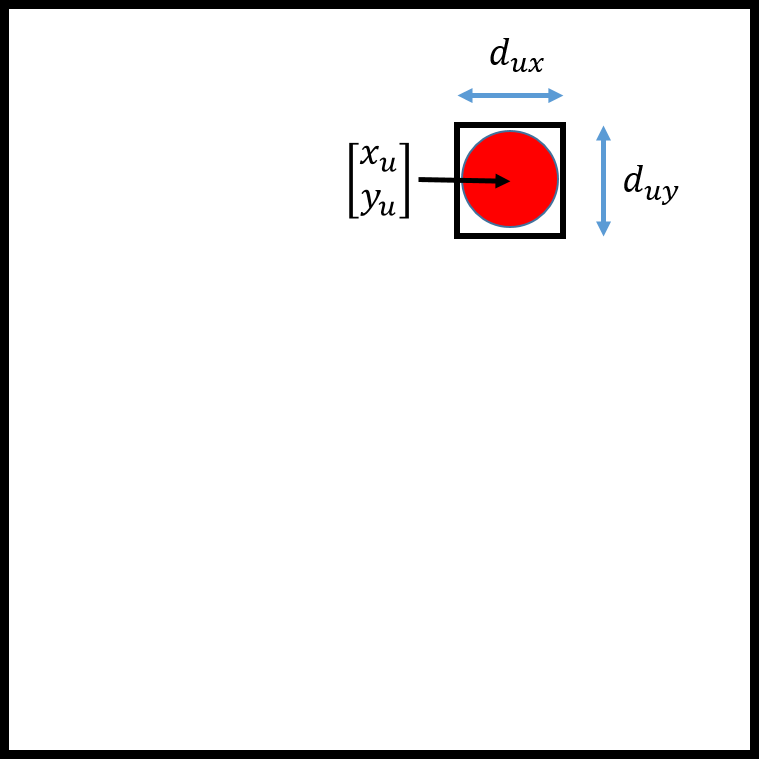
\includegraphics[scale=0.4]{cameraMeasurement}
\end{center}

\medskip

These measurements are related to the hidden state $\bf{\vec{x_C}} = 
\mat{ x_C & y_C & z_C }^{T}$ in the following way: 

\[
    \bf{\vec{y}} = h(\bf{\vec{x}})
         = \mat{x_u \\ y_u \\ d_{ux} \\ d_{uy}} 
     = \mat{ \frac{f_x x_c}{z_c} \\ 
             \frac{f_y y_c}{z_c} \\ 
             \frac{d_c}{z_c \sqrt{\frac{1}{f_x^{2}} + \frac{1}{f_y^{2}}}} \\
             \frac{d_c}{z_c \sqrt{\frac{1}{f_x^{2}} + \frac{1}{f_y^{2}}}}
           }
\]

\end{flushleft}

\end{document}
